\section{Databases} % (fold)
\label{tech:sec:databases}
A database collects data, either records or files. From the Rails perspective, this can either be a schema-based or a schema-less database.


\subsection{MySQL}
MySQL is the most popular open source database in the world, having consistently fast performance, high reliability and ease of use~\cite{why_mysql}. It was first released in 1995 and it is the default database on a Ruby on Rails project. This is the database of choice for all \textit{37signals}'s applications~\cite{interview_dhh}.  It is a relational schema-based database that offers useful features like various storage engines, transactions, indexes, load balancing and so on.

Figure~\ref{fig:mysql_architecture} presents a simple overview over MySQL's architecture.
\begin{figure}[h]
  \centering
    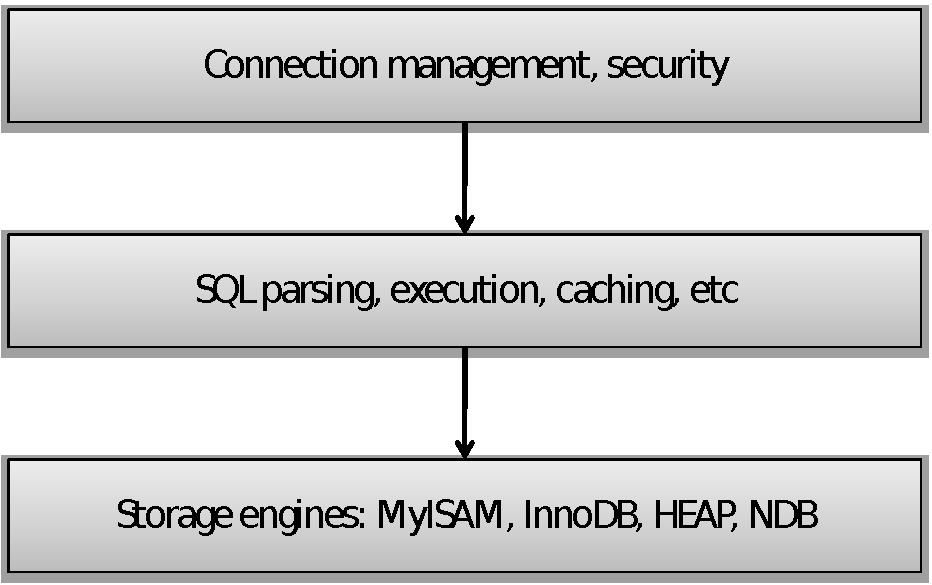
\includegraphics[width=0.75\textwidth]{mysql_architecture}
  \caption{Logical view of MySQL's architecture}
  \label{fig:mysql_architecture}
\end{figure}
The top layer is related with the services that are not unique to MySQL, like connection handling, authentication and security. The middle layer refers to crucial MySQL features like query parsing, analysis, optimization, caching and all the built-in functions.  This layer also holds all functionality across storage engines and stored procedures. Finally, the bottom layer consists in the storage engines themselves, responsible for the storage and retrieval of all stored data~\cite{high_performance_mysql}. MySQL has four main storage engines, all with advantages and disadvantages, the default one being InnoDB.

A high-level summary of the characteristics of all four storage engines can be found on table~\ref{tab:storage_engines_mysql}.
\begin{table}[ht]
  \centering
  
  \begin{tabular}{p{4cm}|p{2cm}|p{2cm}|p{3cm}|p{2cm}}
    \textsc{Attribute}
  & \textsc{MyISAM}
  & \textsc{Heap}
  & \textsc{BDB}
  & \textsc{InnoDB} \\
  \hline

    \textbf{Transactions}
  & No
  & No
  & Yes
  & Yes \\

  \hline
    \textbf{Lock granularity}
  & Table
  & Table
  & Page
  & Row \\

  \hline
    \textbf{Storage}
  & Split files
  & In-memory
  & Single file per table
  & Tablespace \\

  \hline
    \textbf{Isolation levels}
  & None
  & None
  & Read committed
  & All \\

  \hline
    \textbf{Portable format}
  & Yes
  & No
  & No
  & Yes \\

  \hline
    \textbf{Referential integrity}
  & No
  & No
  & No
  & Yes \\

  \hline
    \textbf{Primary key with data}
  & No
  & No
  & Yes
  & Yes \\
    
  \hline
    \textbf{MySQL caching}
  & No
  & Yes
  & Yes
  & Yes \\

  \hline
    \textbf{Available versions}
  & All versions
  & All versions
  & MySQL-Max
  & All versions \\
  \end{tabular}
  \caption{Storage engine characteristics in MySQL}
  \label{tab:storage_engines_mysql}
\end{table}
Rails' ActiveRecord natively supports this type of database.


\subsection{PostgreSQL}
PostgreSQL is the most advanced open source database server. It was started by Michael Stonebraker at the University of California in Berkeley and had its first release in 1989. It is a DBMS that contains all the features found on other open source or commercial databases and a few more. Some of these features include~\cite{beginning_postgresql}:
\begin{itemize}
  \item Transactions;
  \item Subselects;
  \item Views;
  \item Foreign key referential integrity;
  \item Sophisticated locking;
  \item User-defined types;
  \item Inheritance;
  \item Rules;
  \item Multiple-version concurrency control;
  \item Native Microsoft Windows version;
  \item Table spaces;
  \item Ability to alter column types;
  \item  Point-in-time recovery.
\end{itemize}
PostgreSQL has some prominent users, like MySpace, who strengthen its credibility as a full-featured scalable highly-reliable relational database~\cite{petabyte_warehouses}. Rails' ActiveRecord natively supports this type of database.


\subsection{MongoDB}
MongoDB is a scalable, high performance, open source, schema-free, document-oriented database written in C++ whose first release was in early 2009. It is a combination of key-value stores, fast and highly scalable, and traditional RDBMS systems which provide structured schemas and powerful queries. Among other features, MongoDB provides~\cite{mongodb}:
\begin{itemize}
  \item Document-oriented storage (the simplicity and power of JSON-like data schemas);
  \item Dynamic queries;
  \item Full index support, extending to inner-objects and embedded arrays;
  \item Query profiling;
  \item Fast, in-place updates;
  \item Efficient storage of binary data large objects (e.g. photos and videos);
  \item Replication and fail-over support;
  \item Auto-sharding for cloud-level scalability;
  \item MapReduce for complex aggregation.
\end{itemize}
This database has been gaining popularity within the Rails community for its simplicity of use, high performance and many features that fit well within the Ruby development  philosophy~\cite{mongodb_rails}. Mongo is very performance oriented and some of its features that provide outstanding performance are~\cite{mongodb_couchdb}:
\begin{itemize}
  \item Client driver per language: native socket protocol for client/server interface (not REST);
  \item Use of memory mapped files for data storage;
  \item Collection-oriented storage (objects from the same collection are stored contiguously);
  \item Update-in-place (not MVCC);
  \item Written in C++.
\end{itemize}
Rails' ActiveRecord does not natively support MongoDB. For its usage in Rails the developer must use \textit{MongoMapper}, which provides access to Mongo database operations and natively supports Ruby objects without conversions~\cite{mongomapper}.

